\section{Generowanie labiryntu}

Do generowania labiryntów kluczowe jest zrozumienie idei drzew rozpinających.

\textbf{Drzewo rozpinające} \cite{cormen2009} to taki podgraf oryginalnego grafu, który zawiera wszystkie jego wierzchołki, a jednocześnie jest spójny i nie zawiera cykli. 

\textbf{Spójność grafu} \cite{balakrishnan2005} oznacza, że między każdą parą wierzchołków istnieje co najmniej jedna ścieżka, czyli można przejść z dowolnego wierzchołka do dowolnego innego, poruszając się po krawędziach grafu. Różnicę między grafem spójnym oraz niespójnym przedstawia rysunek~\ref{fig:connected_and_not_connected_graph}.

\begin{figure}[H]
    \centering
    \begin{subfigure}{0.4\textwidth}
        \centering
        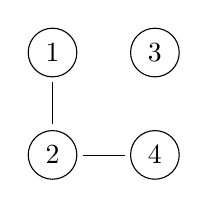
\begin{tikzpicture}[scale=1, every node/.style={circle,draw,minimum size=5mm}]
            \node (n0) at (0,1.3) {1};
            \node (n1) at (0,0) {2};
            \node (n2) at (1.3,1.3) {3};
            \node (n3) at (1.3,0) {4};
            \draw[very thin, black] (0,0.39) -- (0,0.92);
            \draw[very thin, black] (0,0.39) -- (0,0.92);
            \draw[very thin, black] (0.39,0) -- (0.92,0);
        \end{tikzpicture}
        \caption{Graf niespójny.}
        \label{fig:connected_and_not_connected_graph_a}
    \end{subfigure}
    \begin{subfigure}{0.4\textwidth}
        \centering
        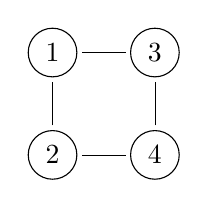
\begin{tikzpicture}[scale=1, every node/.style={circle,draw,minimum size=5mm}]
            \node (n0) at (0,1.3) {1};
            \node (n1) at (0,0) {2};
            \node (n2) at (1.3,1.3) {3};
            \node (n3) at (1.3,0) {4};
            \draw[very thin, black] (0,0.375) -- (0,0.93);
            \draw[very thin, black] (1.3,0.375) -- (1.3,0.93);
            \draw[very thin, black] (0.375,0) -- (0.93,0);
            \draw[very thin, black] (0.375,1.3) -- (0.93,1.3);
        \end{tikzpicture}
        \caption{Graf spójny.}
        \label{fig:connected_and_not_connected_graph_b}
    \end{subfigure}
    \caption{Przykłady grafów spójnych i niespójnych.}
    \label{fig:connected_and_not_connected_graph}
\end{figure}

\textbf{Cyklem} \cite{balakrishnan2005} nazywamy ścieżkę zaczynającą się i kończącą w tym samym wierzchołku, w której żadna krawędź ani wierzchołek (poza początkiem i końcem) się nie powtarza. Obecność cykli oznacza, że można okrążyć pewien obszar grafu i wrócić do punktu startu inną drogą, co w kontekście labiryntu oznacza istnienie pętli. W drzewie rozpinającym takich pętli nie ma, co gwarantuje unikalną ścieżkę między dowolnymi dwoma wierzchołkami. Przykładowy graf zawierający cykl został pokazany na rysunku \ref{fig:graph_cycle}.

\begin{figure}[H]
    \centering
        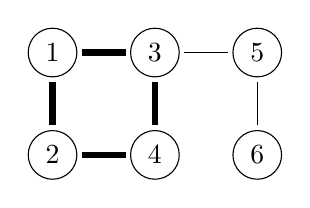
\begin{tikzpicture}[scale=1, every node/.style={circle,draw,minimum size=5mm}]
            \node (n0) at (0,1.3) {1};
            \node (n1) at (0,0) {2};
            \node (n2) at (1.3,1.3) {3};
            \node (n3) at (1.3,0) {4};
            \node (n3) at (2.6,1.3) {5};
            \node (n3) at (2.6,0) {6};
            
            \draw[line width=0.8mm, black] (0,0.375) -- (0,0.93);
            \draw[line width=0.8mm, black] (1.3,0.375) -- (1.3,0.93);
            \draw[line width=0.8mm, black] (0.375,0) -- (0.93,0);
            \draw[line width=0.8mm, black] (0.375,1.3) -- (0.93,1.3);
            \draw[very thin, black] (1.675,1.3) -- (2.23,1.3);
            \draw[very thin, black] (2.6,0.375) -- (2.6,0.93);
        \end{tikzpicture}
    \caption{Graf zawierający cykl (pogrubiona linia).}
    \label{fig:graph_cycle}
\end{figure}

\textbf{Minimalne drzewo rozpinające} \cite{cormen2009} (ang. \textit{MST, minimum spanning tree}) to takie drzewo rozpinające, dla którego suma wag krawędzi jest najmniejsza spośród wszystkich możliwych drzew rozpinających danego grafu. W grafach nieważonych, jak te stosowane przy modelowaniu labiryntów, wszystkie krawędzie są traktowane jako równe, dlatego każde drzewo rozpinające o minimalnej liczbie krawędzi spełnia warunki \textit{MST}. Przykładowe minimalne drzewo rozpinające dla grafu z równoważnymi krawędziami pokazuje rysunek \ref{fig:minimum_spanning_tree}.

\begin{figure}[H]
    \centering
    \begin{subfigure}{0.45\textwidth}
        \centering
        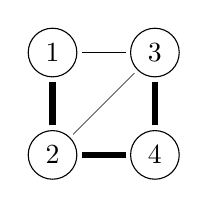
\begin{tikzpicture}[scale=1, every node/.style={circle,draw,minimum size=5mm}]
            \node (n0) at (0,1.3) {1};
            \node (n1) at (0,0) {2};
            \node (n2) at (1.3,1.3) {3};
            \node (n3) at (1.3,0) {4};
            \draw[line width=0.8mm, black] (0,0.375) -- (0,0.93);
            \draw[line width=0.8mm, black] (1.3,0.375) -- (1.3,0.93);
            \draw[line width=0.8mm, black] (0.375,0) -- (0.93,0);
            \draw[very thin, black] (0.375,1.3) -- (0.93,1.3);
            \draw[very thin, black] (0.26,0.26) -- (1.04,1.04);
        \end{tikzpicture}
        \caption{\centering Ścieżka będąca minimalnym drzewem rozpinającym (3 kroki).}
        \label{fig:minimum_spanning_tree_a}
    \end{subfigure}
    \begin{subfigure}{0.45\textwidth}
        \centering
        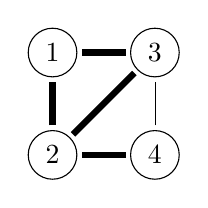
\begin{tikzpicture}[scale=1, every node/.style={circle,draw,minimum size=5mm}]
            \node (n0) at (0,1.3) {1};
            \node (n1) at (0,0) {2};
            \node (n2) at (1.3,1.3) {3};
            \node (n3) at (1.3,0) {4};
            \draw[line width=0.8mm, black] (0,0.375) -- (0,0.93);
            \draw[very thin, black] (1.3,0.375) -- (1.3,0.93);
            \draw[line width=0.8mm, black] (0.375,0) -- (0.93,0);
            \draw[line width=0.8mm, black] (0.375,1.3) -- (0.93,1.3);
            \draw[line width=0.8mm, black] (0.26,0.26) -- (1.04,1.04);
        \end{tikzpicture}
        \caption{\centering Ścieżka nie stanowiąca minimalnego drzewa rozpinającego (4 kroki).}
        \label{fig:minimum_spanning_tree_b}
    \end{subfigure}
    \caption{Ścieżki spełniające oraz nie spełniające założeń \textit{MST} (pogrubione linie).}
    \label{fig:minimum_spanning_tree}
\end{figure}

Algorytmy generujące labirynty sprowadzają się właśnie do wyznaczenia wspomnianego drzewa rozpinającego. 
Uzyskane drzewo określa, które krawędzie (ścieżki) są dostępne, a które stanowią ściany labiryntu.

\subsection{Algorytm Prima}

Algorytm Prima w kontekście generowania labiryntu działa poprzez stopniowe budowanie połączeń między komórkami planszy. W każdej iteracji wybierana jest losowa krawędź prowadząca z odwiedzonej komórki do jednej z sąsiednich, jeszcze nieodwiedzonych. Wybrana komórka zostaje następnie połączona z dotychczasowym obszarem labiryntu. Proces ten powtarzany jest aż do momentu, gdy wszystkie komórki zostaną połączone, tworząc spójną strukturę bez cykli. Szczegółowy przebieg algorytmu wygląda następująco:

\begin{enumerate}
    \item Na początku tworzona jest plansza, w której wszystkie komórki są oznaczone jako ściany. Rysunek \ref{fig:prim_step_1} przedstawia początkowy układ planszy w całości wypełnionej ścianami.
    
    \begin{figure}[ht]
    \centering
    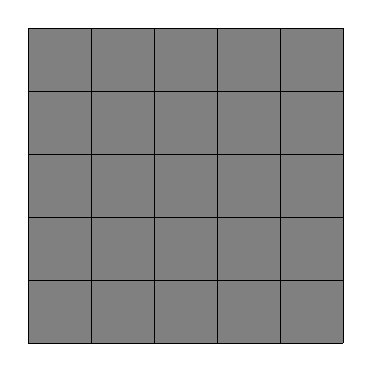
\begin{tikzpicture}[scale=0.8]
        \foreach \x in {0,...,4} {
            \foreach \y in {0,...,4} {
                \fill[gray] (\x,\y) rectangle ++(1,1);
            }
        }
        \draw[step=1cm,ultra thin,black] (0,0) grid (5,5);
    \end{tikzpicture}
    \caption{\centering Cała plansza stanowi ściany.}
    \label{fig:prim_step_1}
\end{figure}

    \item Następnie wybierane jest losowe pole, które zostaje oznaczone jako przejście. Rysunek \ref{fig:prim_step_2} przedstawia wybrane losowo pole startowe.
    
    \begin{figure}[H]
    \centering
    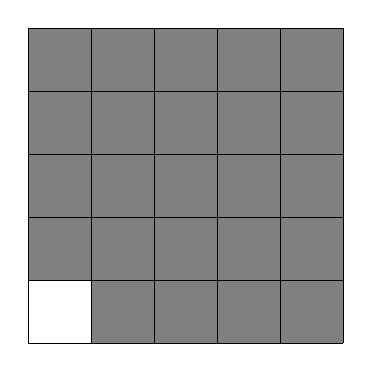
\begin{tikzpicture}[scale=0.8]
        \foreach \x in {0,...,4} {
            \foreach \y in {0,...,4} {
                \fill[gray] (\x,\y) rectangle ++(1,1);
            }
        }
        \fill[white] (0, 0) rectangle ++(1,1);
        \draw[step=1cm,ultra thin,black] (0,0) grid (5,5);
    \end{tikzpicture}
    \caption{\centering Losowe pole startowe.}
    \label{fig:prim_step_2}
\end{figure}

    \item Do zbioru krawędzi dodawane są sąsiednie komórki, do których można przejść bezpośrednio z pola startowego. Za sąsiednie uznaje się komórki oddalone o jedno pole w pionie lub poziomie. Ilustrację tego etapu przedstawiono na Rysunku \ref{fig:prim_step_3}.
    
    \begin{figure}[h]
    \centering
    \begin{tikzpicture}[scale=0.8]
        \foreach \x in {0,...,4} {
            \foreach \y in {0,...,4} {
                \fill[gray] (\x,\y) rectangle ++(1,1);
            }
        }

        \fill[white] (0,2) rectangle ++(1,1);
        \fill[pattern=north east lines, pattern color=black] (0,2) rectangle ++(1,1);

        \fill[white] (2,0) rectangle ++(1,1);
        \fill[pattern=north east lines, pattern color=black] (2,0) rectangle ++(1,1);

        \fill[white] (0, 0) rectangle ++(1,1);

        \draw[step=1cm,ultra thin,black] (0,0) grid (5,5);
    \end{tikzpicture}
    \caption{\centering  Wybór sąsiednich pól.}
    \label{fig:prim_step_3}
\end{figure}

    \item Losowana jest jedna krawędź ze zbioru potencjalnych przejść. Jeśli prowadzi ona do nieodwiedzonego pola, tworzy się przejście między bieżącym polem a nowym (usuwana jest ściana między nimi), a nowe pole zostaje oznaczone jako przejście. Następnie do zbioru krawędzi dodawani są sąsiedzi nowo odwiedzonego pola. Ilustrację tego etapu przedstawiono na Rysunku \ref{fig:prim_step_4}.

    \begin{figure}[H]
    \centering
    \begin{tikzpicture}[scale=0.8]
        \foreach \x in {0,...,4} {
            \foreach \y in {0,...,4} {
                \fill[gray] (\x,\y) rectangle ++(1,1);
            }
        }

        \fill[white] (0,2) rectangle ++(1,1);
        \fill[pattern=north east lines, pattern color=black] (0,2) rectangle ++(1,1);

        \fill[white] (2,2) rectangle ++(1,1);
        \fill[pattern=north east lines, pattern color=black] (2,2) rectangle ++(1,1);

        \fill[white] (4,0) rectangle ++(1,1);
        \fill[pattern=north east lines, pattern color=black] (4,0) rectangle ++(1,1);


        \fill[white] (0, 0) rectangle ++(1,1);
        \fill[white] (2, 0) rectangle ++(1,1);
        \fill[white] (1, 0) rectangle ++(1,1);
        \draw[->, very thick, black] (0.5,0.5) -- (2.5,0.5);

        \draw[step=1cm,ultra thin,black] (0,0) grid (5,5);
    \end{tikzpicture}
    \caption{\centering Utworzenie krawędzi do sąsiedniego pola.}
    \label{fig:prim_step_4}
\end{figure}

    \item Proces powtarza się, aż zbiór krawędzi stanie się pusty, co oznacza, że wszystkie komórki zostały połączone.

    Na Rysunku \ref{fig:prim_later_steps_a} przedstawiono wyznaczanie kolejnych krawędzi labiryntu, a na Rysunku \ref{fig:prim_later_steps_b} końcowy labirynt powstały na podstawie tych krawędzi.
    
    \begin{figure}[ht]
    \centering
    \begin{subfigure}{0.45\textwidth}
        \centering
        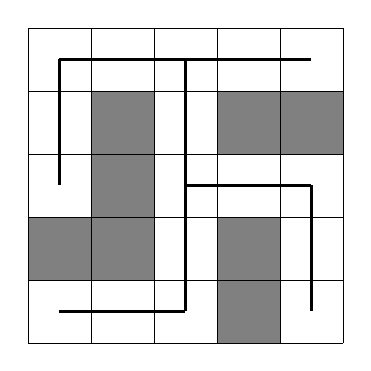
\begin{tikzpicture}[scale=0.8, every node/.style={circle,draw,minimum size=8mm}]
            \draw[very thick, black] (0.5,0.5) -- (2.5,0.5);
            \draw[very thick, black] (2.5,0.5) -- (2.5,4.5);
            \draw[very thick, black] (0.5,4.5) -- (4.5,4.5);
            \draw[very thick, black] (0.5,4.5) -- (0.5,2.5);
            \draw[very thick, black] (4.5,2.5) -- (4.5,0.5);
            \draw[very thick, black] (2.5,2.5) -- (4.5,2.5);

            \fill[gray] (0, 1) rectangle ++(1,1);
            \fill[gray] (1, 1) rectangle ++(1,1);
            \fill[gray] (1, 2) rectangle ++(1,1);
            \fill[gray] (1, 3) rectangle ++(1,1);
            \fill[gray] (3, 3) rectangle ++(1,1);
            \fill[gray] (4, 3) rectangle ++(1,1);
            \fill[gray] (3, 0) rectangle ++(1,1);
            \fill[gray] (3, 1) rectangle ++(1,1);

            \draw[step=1cm,ultra thin,black] (0,0) grid (5,5);
        \end{tikzpicture}
        \caption{\centering Wyznaczanie kolejnych krawędzi labiryntu.}
        \label{fig:prim_later_steps_a}
    \end{subfigure}
    \begin{subfigure}{0.45\textwidth}
        \centering
        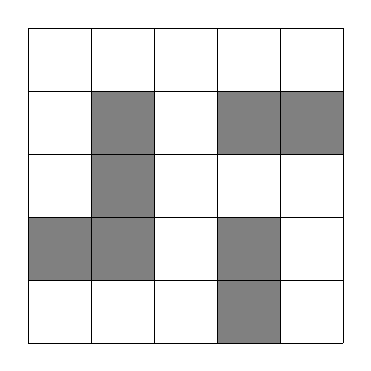
\begin{tikzpicture}[scale=0.8, every node/.style={circle,draw,minimum size=8mm}]
            \fill[gray] (0, 1) rectangle ++(1,1);
            \fill[gray] (1, 1) rectangle ++(1,1);
            \fill[gray] (1, 2) rectangle ++(1,1);
            \fill[gray] (1, 3) rectangle ++(1,1);
            \fill[gray] (3, 3) rectangle ++(1,1);
            \fill[gray] (4, 3) rectangle ++(1,1);
            \fill[gray] (3, 0) rectangle ++(1,1);
            \fill[gray] (3, 1) rectangle ++(1,1);

            \draw[step=1cm,ultra thin,black] (0,0) grid (5,5);
        \end{tikzpicture}
        \caption{\centering Labirynt powstały na podstawie wyznaczonych krawędzi.}
        \label{fig:prim_later_steps_b}
    \end{subfigure}
    \caption{Kolejne kroki działania algorytmu.}
    \label{fig:prim_later_steps}
\end{figure}
\end{enumerate}

\subsection{Algorytm Prima}

Algorytm Prima w kontekście generowania labiryntu działa poprzez stopniowe budowanie połączeń między komórkami planszy. W każdej iteracji wybierana jest losowa krawędź prowadząca z odwiedzonej komórki do jednej z sąsiednich, jeszcze nieodwiedzonych. Wybrana komórka zostaje następnie połączona z dotychczasowym obszarem labiryntu. Proces ten powtarzany jest aż do momentu, gdy wszystkie komórki zostaną połączone, tworząc spójną strukturę bez cykli. Szczegółowy przebieg algorytmu wygląda następująco:

\begin{enumerate}
    \item Na początku tworzona jest plansza, w której wszystkie komórki są oznaczone jako ściany. Rysunek \ref{fig:prim_step_1} przedstawia początkowy układ planszy w całości wypełnionej ścianami.
    
    \begin{figure}[ht]
    \centering
    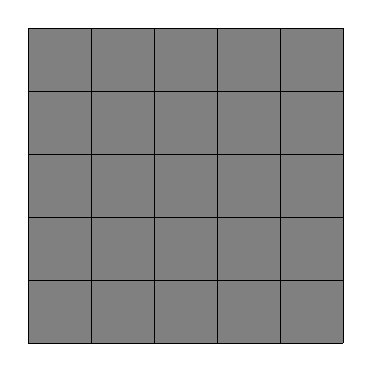
\begin{tikzpicture}[scale=0.8]
        \foreach \x in {0,...,4} {
            \foreach \y in {0,...,4} {
                \fill[gray] (\x,\y) rectangle ++(1,1);
            }
        }
        \draw[step=1cm,ultra thin,black] (0,0) grid (5,5);
    \end{tikzpicture}
    \caption{\centering Cała plansza stanowi ściany.}
    \label{fig:prim_step_1}
\end{figure}

    \item Następnie wybierane jest losowe pole, które zostaje oznaczone jako przejście. Rysunek \ref{fig:prim_step_2} przedstawia wybrane losowo pole startowe.
    
    \begin{figure}[H]
    \centering
    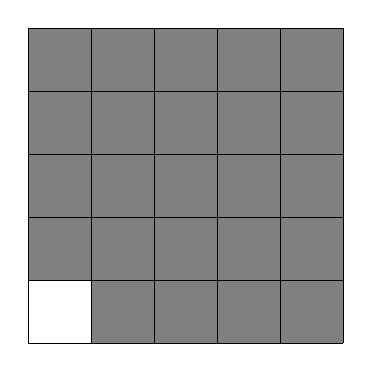
\begin{tikzpicture}[scale=0.8]
        \foreach \x in {0,...,4} {
            \foreach \y in {0,...,4} {
                \fill[gray] (\x,\y) rectangle ++(1,1);
            }
        }
        \fill[white] (0, 0) rectangle ++(1,1);
        \draw[step=1cm,ultra thin,black] (0,0) grid (5,5);
    \end{tikzpicture}
    \caption{\centering Losowe pole startowe.}
    \label{fig:prim_step_2}
\end{figure}

    \item Do zbioru krawędzi dodawane są sąsiednie komórki, do których można przejść bezpośrednio z pola startowego. Za sąsiednie uznaje się komórki oddalone o jedno pole w pionie lub poziomie. Ilustrację tego etapu przedstawiono na Rysunku \ref{fig:prim_step_3}.
    
    \begin{figure}[h]
    \centering
    \begin{tikzpicture}[scale=0.8]
        \foreach \x in {0,...,4} {
            \foreach \y in {0,...,4} {
                \fill[gray] (\x,\y) rectangle ++(1,1);
            }
        }

        \fill[white] (0,2) rectangle ++(1,1);
        \fill[pattern=north east lines, pattern color=black] (0,2) rectangle ++(1,1);

        \fill[white] (2,0) rectangle ++(1,1);
        \fill[pattern=north east lines, pattern color=black] (2,0) rectangle ++(1,1);

        \fill[white] (0, 0) rectangle ++(1,1);

        \draw[step=1cm,ultra thin,black] (0,0) grid (5,5);
    \end{tikzpicture}
    \caption{\centering  Wybór sąsiednich pól.}
    \label{fig:prim_step_3}
\end{figure}

    \item Losowana jest jedna krawędź ze zbioru potencjalnych przejść. Jeśli prowadzi ona do nieodwiedzonego pola, tworzy się przejście między bieżącym polem a nowym (usuwana jest ściana między nimi), a nowe pole zostaje oznaczone jako przejście. Następnie do zbioru krawędzi dodawani są sąsiedzi nowo odwiedzonego pola. Ilustrację tego etapu przedstawiono na Rysunku \ref{fig:prim_step_4}.

    \begin{figure}[H]
    \centering
    \begin{tikzpicture}[scale=0.8]
        \foreach \x in {0,...,4} {
            \foreach \y in {0,...,4} {
                \fill[gray] (\x,\y) rectangle ++(1,1);
            }
        }

        \fill[white] (0,2) rectangle ++(1,1);
        \fill[pattern=north east lines, pattern color=black] (0,2) rectangle ++(1,1);

        \fill[white] (2,2) rectangle ++(1,1);
        \fill[pattern=north east lines, pattern color=black] (2,2) rectangle ++(1,1);

        \fill[white] (4,0) rectangle ++(1,1);
        \fill[pattern=north east lines, pattern color=black] (4,0) rectangle ++(1,1);


        \fill[white] (0, 0) rectangle ++(1,1);
        \fill[white] (2, 0) rectangle ++(1,1);
        \fill[white] (1, 0) rectangle ++(1,1);
        \draw[->, very thick, black] (0.5,0.5) -- (2.5,0.5);

        \draw[step=1cm,ultra thin,black] (0,0) grid (5,5);
    \end{tikzpicture}
    \caption{\centering Utworzenie krawędzi do sąsiedniego pola.}
    \label{fig:prim_step_4}
\end{figure}

    \item Proces powtarza się, aż zbiór krawędzi stanie się pusty, co oznacza, że wszystkie komórki zostały połączone.

    Na Rysunku \ref{fig:prim_later_steps_a} przedstawiono wyznaczanie kolejnych krawędzi labiryntu, a na Rysunku \ref{fig:prim_later_steps_b} końcowy labirynt powstały na podstawie tych krawędzi.
    
    \begin{figure}[ht]
    \centering
    \begin{subfigure}{0.45\textwidth}
        \centering
        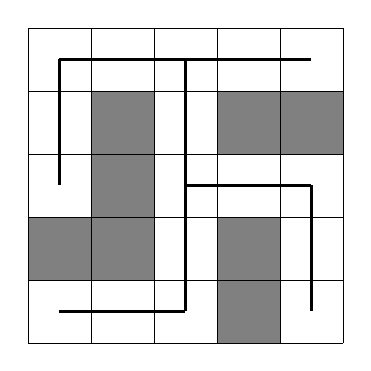
\begin{tikzpicture}[scale=0.8, every node/.style={circle,draw,minimum size=8mm}]
            \draw[very thick, black] (0.5,0.5) -- (2.5,0.5);
            \draw[very thick, black] (2.5,0.5) -- (2.5,4.5);
            \draw[very thick, black] (0.5,4.5) -- (4.5,4.5);
            \draw[very thick, black] (0.5,4.5) -- (0.5,2.5);
            \draw[very thick, black] (4.5,2.5) -- (4.5,0.5);
            \draw[very thick, black] (2.5,2.5) -- (4.5,2.5);

            \fill[gray] (0, 1) rectangle ++(1,1);
            \fill[gray] (1, 1) rectangle ++(1,1);
            \fill[gray] (1, 2) rectangle ++(1,1);
            \fill[gray] (1, 3) rectangle ++(1,1);
            \fill[gray] (3, 3) rectangle ++(1,1);
            \fill[gray] (4, 3) rectangle ++(1,1);
            \fill[gray] (3, 0) rectangle ++(1,1);
            \fill[gray] (3, 1) rectangle ++(1,1);

            \draw[step=1cm,ultra thin,black] (0,0) grid (5,5);
        \end{tikzpicture}
        \caption{\centering Wyznaczanie kolejnych krawędzi labiryntu.}
        \label{fig:prim_later_steps_a}
    \end{subfigure}
    \begin{subfigure}{0.45\textwidth}
        \centering
        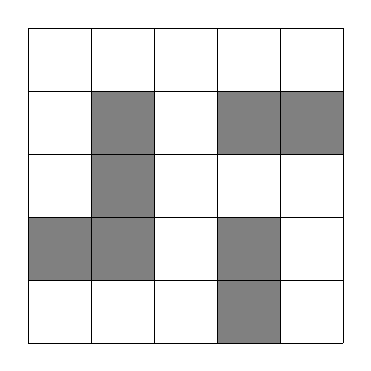
\begin{tikzpicture}[scale=0.8, every node/.style={circle,draw,minimum size=8mm}]
            \fill[gray] (0, 1) rectangle ++(1,1);
            \fill[gray] (1, 1) rectangle ++(1,1);
            \fill[gray] (1, 2) rectangle ++(1,1);
            \fill[gray] (1, 3) rectangle ++(1,1);
            \fill[gray] (3, 3) rectangle ++(1,1);
            \fill[gray] (4, 3) rectangle ++(1,1);
            \fill[gray] (3, 0) rectangle ++(1,1);
            \fill[gray] (3, 1) rectangle ++(1,1);

            \draw[step=1cm,ultra thin,black] (0,0) grid (5,5);
        \end{tikzpicture}
        \caption{\centering Labirynt powstały na podstawie wyznaczonych krawędzi.}
        \label{fig:prim_later_steps_b}
    \end{subfigure}
    \caption{Kolejne kroki działania algorytmu.}
    \label{fig:prim_later_steps}
\end{figure}
\end{enumerate}

\subsection{Algorytm Prima}

Algorytm Prima w kontekście generowania labiryntu działa poprzez stopniowe budowanie połączeń między komórkami planszy. W każdej iteracji wybierana jest losowa krawędź prowadząca z odwiedzonej komórki do jednej z sąsiednich, jeszcze nieodwiedzonych. Wybrana komórka zostaje następnie połączona z dotychczasowym obszarem labiryntu. Proces ten powtarzany jest aż do momentu, gdy wszystkie komórki zostaną połączone, tworząc spójną strukturę bez cykli. Szczegółowy przebieg algorytmu wygląda następująco:

\begin{enumerate}
    \item Na początku tworzona jest plansza, w której wszystkie komórki są oznaczone jako ściany. Rysunek \ref{fig:prim_step_1} przedstawia początkowy układ planszy w całości wypełnionej ścianami.
    
    \begin{figure}[ht]
    \centering
    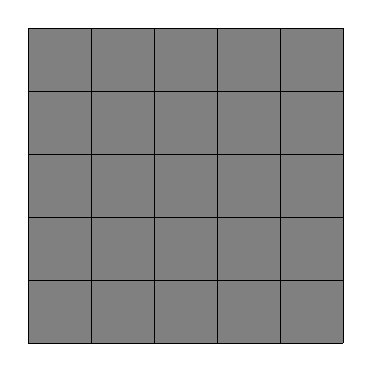
\begin{tikzpicture}[scale=0.8]
        \foreach \x in {0,...,4} {
            \foreach \y in {0,...,4} {
                \fill[gray] (\x,\y) rectangle ++(1,1);
            }
        }
        \draw[step=1cm,ultra thin,black] (0,0) grid (5,5);
    \end{tikzpicture}
    \caption{\centering Cała plansza stanowi ściany.}
    \label{fig:prim_step_1}
\end{figure}

    \item Następnie wybierane jest losowe pole, które zostaje oznaczone jako przejście. Rysunek \ref{fig:prim_step_2} przedstawia wybrane losowo pole startowe.
    
    \begin{figure}[H]
    \centering
    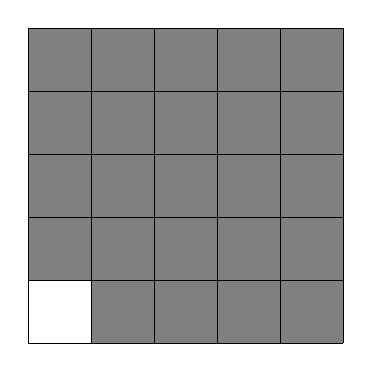
\begin{tikzpicture}[scale=0.8]
        \foreach \x in {0,...,4} {
            \foreach \y in {0,...,4} {
                \fill[gray] (\x,\y) rectangle ++(1,1);
            }
        }
        \fill[white] (0, 0) rectangle ++(1,1);
        \draw[step=1cm,ultra thin,black] (0,0) grid (5,5);
    \end{tikzpicture}
    \caption{\centering Losowe pole startowe.}
    \label{fig:prim_step_2}
\end{figure}

    \item Do zbioru krawędzi dodawane są sąsiednie komórki, do których można przejść bezpośrednio z pola startowego. Za sąsiednie uznaje się komórki oddalone o jedno pole w pionie lub poziomie. Ilustrację tego etapu przedstawiono na Rysunku \ref{fig:prim_step_3}.
    
    \begin{figure}[h]
    \centering
    \begin{tikzpicture}[scale=0.8]
        \foreach \x in {0,...,4} {
            \foreach \y in {0,...,4} {
                \fill[gray] (\x,\y) rectangle ++(1,1);
            }
        }

        \fill[white] (0,2) rectangle ++(1,1);
        \fill[pattern=north east lines, pattern color=black] (0,2) rectangle ++(1,1);

        \fill[white] (2,0) rectangle ++(1,1);
        \fill[pattern=north east lines, pattern color=black] (2,0) rectangle ++(1,1);

        \fill[white] (0, 0) rectangle ++(1,1);

        \draw[step=1cm,ultra thin,black] (0,0) grid (5,5);
    \end{tikzpicture}
    \caption{\centering  Wybór sąsiednich pól.}
    \label{fig:prim_step_3}
\end{figure}

    \item Losowana jest jedna krawędź ze zbioru potencjalnych przejść. Jeśli prowadzi ona do nieodwiedzonego pola, tworzy się przejście między bieżącym polem a nowym (usuwana jest ściana między nimi), a nowe pole zostaje oznaczone jako przejście. Następnie do zbioru krawędzi dodawani są sąsiedzi nowo odwiedzonego pola. Ilustrację tego etapu przedstawiono na Rysunku \ref{fig:prim_step_4}.

    \begin{figure}[H]
    \centering
    \begin{tikzpicture}[scale=0.8]
        \foreach \x in {0,...,4} {
            \foreach \y in {0,...,4} {
                \fill[gray] (\x,\y) rectangle ++(1,1);
            }
        }

        \fill[white] (0,2) rectangle ++(1,1);
        \fill[pattern=north east lines, pattern color=black] (0,2) rectangle ++(1,1);

        \fill[white] (2,2) rectangle ++(1,1);
        \fill[pattern=north east lines, pattern color=black] (2,2) rectangle ++(1,1);

        \fill[white] (4,0) rectangle ++(1,1);
        \fill[pattern=north east lines, pattern color=black] (4,0) rectangle ++(1,1);


        \fill[white] (0, 0) rectangle ++(1,1);
        \fill[white] (2, 0) rectangle ++(1,1);
        \fill[white] (1, 0) rectangle ++(1,1);
        \draw[->, very thick, black] (0.5,0.5) -- (2.5,0.5);

        \draw[step=1cm,ultra thin,black] (0,0) grid (5,5);
    \end{tikzpicture}
    \caption{\centering Utworzenie krawędzi do sąsiedniego pola.}
    \label{fig:prim_step_4}
\end{figure}

    \item Proces powtarza się, aż zbiór krawędzi stanie się pusty, co oznacza, że wszystkie komórki zostały połączone.

    Na Rysunku \ref{fig:prim_later_steps_a} przedstawiono wyznaczanie kolejnych krawędzi labiryntu, a na Rysunku \ref{fig:prim_later_steps_b} końcowy labirynt powstały na podstawie tych krawędzi.
    
    \begin{figure}[ht]
    \centering
    \begin{subfigure}{0.45\textwidth}
        \centering
        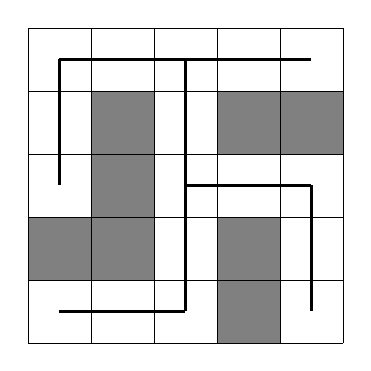
\begin{tikzpicture}[scale=0.8, every node/.style={circle,draw,minimum size=8mm}]
            \draw[very thick, black] (0.5,0.5) -- (2.5,0.5);
            \draw[very thick, black] (2.5,0.5) -- (2.5,4.5);
            \draw[very thick, black] (0.5,4.5) -- (4.5,4.5);
            \draw[very thick, black] (0.5,4.5) -- (0.5,2.5);
            \draw[very thick, black] (4.5,2.5) -- (4.5,0.5);
            \draw[very thick, black] (2.5,2.5) -- (4.5,2.5);

            \fill[gray] (0, 1) rectangle ++(1,1);
            \fill[gray] (1, 1) rectangle ++(1,1);
            \fill[gray] (1, 2) rectangle ++(1,1);
            \fill[gray] (1, 3) rectangle ++(1,1);
            \fill[gray] (3, 3) rectangle ++(1,1);
            \fill[gray] (4, 3) rectangle ++(1,1);
            \fill[gray] (3, 0) rectangle ++(1,1);
            \fill[gray] (3, 1) rectangle ++(1,1);

            \draw[step=1cm,ultra thin,black] (0,0) grid (5,5);
        \end{tikzpicture}
        \caption{\centering Wyznaczanie kolejnych krawędzi labiryntu.}
        \label{fig:prim_later_steps_a}
    \end{subfigure}
    \begin{subfigure}{0.45\textwidth}
        \centering
        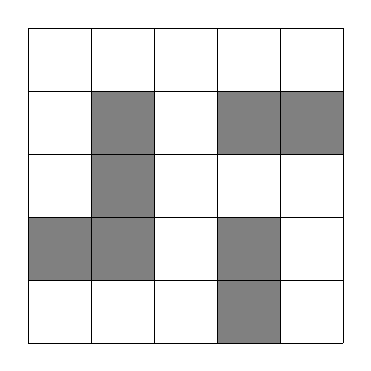
\begin{tikzpicture}[scale=0.8, every node/.style={circle,draw,minimum size=8mm}]
            \fill[gray] (0, 1) rectangle ++(1,1);
            \fill[gray] (1, 1) rectangle ++(1,1);
            \fill[gray] (1, 2) rectangle ++(1,1);
            \fill[gray] (1, 3) rectangle ++(1,1);
            \fill[gray] (3, 3) rectangle ++(1,1);
            \fill[gray] (4, 3) rectangle ++(1,1);
            \fill[gray] (3, 0) rectangle ++(1,1);
            \fill[gray] (3, 1) rectangle ++(1,1);

            \draw[step=1cm,ultra thin,black] (0,0) grid (5,5);
        \end{tikzpicture}
        \caption{\centering Labirynt powstały na podstawie wyznaczonych krawędzi.}
        \label{fig:prim_later_steps_b}
    \end{subfigure}
    \caption{Kolejne kroki działania algorytmu.}
    \label{fig:prim_later_steps}
\end{figure}
\end{enumerate}
